\chapter{Programmazione a Vincoli}\label{capCP}
Come accennato nell'introduzione, la programmazione a vincoli offre un approccio
dichiarativo al programmatore, consentendogli di specificare relazioni tra 
variabili sotto forma di vincoli. Oggigiorno tale
paradigma rappresenta una provata tecnica di ottimizzazione e molti
solver basati su di esso potenziano applicazioni presenti nei settori di 
pianificazione,
configurazione, allocazione di risorse e supporto a decisioni in tempo reale.
Tuttavia l'assenza di una standardizzazione continua a limitarne l'accettazione
nel mondo dell'industria, ed è per ovviare a questa limitazione che è nata
la specifica JSR-331. 

Ma che cos'è effettivamente la programmazione a vincoli? Di cosa si occupa
in pratica? In questo capitolo si darà una definizione formale di problema di 
soddisfacimento di vincoli e si 
vedranno i metodi più comuni di risoluzione. Si vedrà quindi un semplice 
esempio.

\section{Definizione formale}
Un \emph{problema di soddisfacimento di vincoli} (o \emph{CSP}) è definito da un
insieme di variabili e da un insieme di vincoli. Ogni variabile ha un 
dominio non vuoto di possibili valori. Ogni vincolo coinvolge un sottoinsieme
delle variabili e ne specifica le combinazioni di valori possibili.

\begin{defi}
Un \emph{problema di soddisfacimento di vincoli} (o CSP) è una tripla 
$\mathbf{P} = \left\langle \mathbf{V}, \mathbf{D}, \mathbf{C}\right\rangle$
tale che, per ogni $n > 0$ si ha che:
\begin{itemize}
\item[-] $\mathbf{V} = \left\{ X_1, X_2, \ldots, X_n \right\}$ è un insieme
di variabili.
\item[-]$\mathbf{D} = D_1 \times D_2 \times \cdots \times D_n$ è una $n$-upla
di domini tale che $D_i = \textrm{dom}(X_i)$.
\item[-] $\mathbf{C} = \left\{ \mathcal{C}_1, \mathcal{C}_2, \ldots, 
\mathcal{C}_m \right\}$ è un insieme di vincoli di \emph{arità} al più
$n$ definito su un sottoinsieme di $\mathbf{V}$.
\end{itemize}
\end{defi}

Si ha quindi che se un vincolo $\mathcal{C}_i$ ha arità $k$ allora esiste un
insieme di indici $\left\{ i_1, \ldots, i_k \right\} \subseteq 
\left\{ 1, \ldots, n \right\}$ tale che $\mathcal{C}_i \subseteq 
D_{i_1} \times \cdots \times D_{i_k}$.

\begin{defi}Siano $v_1 \in D_1, \ldots, v_n \in D_n$ valori nei
rispettivi domini,
uno \emph{stato} $\mathcal{S}$ del problema $\mathbf{P}$ è definito
dall'assegnamento di valori ad alcune o a tutte le variabili del problema:
\[
\mathcal{S} = \left\{ X_i = v_i, X_j = v_j, \ldots \right\}.
\]
Un assegnamento che non viola nessun vincolo è detto \emph{consistente} o
\emph{legale}. Un assegnamento che coinvolge tutte le variabili del problema
è detto \emph{completo}.
\end{defi}

\begin{defi}
Una \emph{soluzione} del problema è un assegnamento completo e consistente.
\end{defi}

Alcuni CSP richiedono anche che la soluzione massimizzi una \emph{funzione
obiettivo}.

\section{Risoluzione di un CSP}
Per capire in cosa consiste la soluzione di un CSP può essere utile
visualizzarlo come un \emph{grafo di vincoli}, i nodi rappresentano le variabili
del problema e gli archi corrispondono ai vincoli.

Esprimere un problema sotto forma di CSP apporta molti importanti benefici.
Dato che la rappresentazione degli stati è conforme ad un modello accettato,
consistendo sempre in un insieme di variabili con i loro vincoli e domini,
la funzione successore ed il test obiettivo possono essere scritti in un
modo generico che si applica ad ogni CSP. Inoltre è possibile sviluppare
euristiche efficaci che non richiedano esperienza aggiuntiva del dominio.

\begin{figure}\label{figAustralia}
\centering
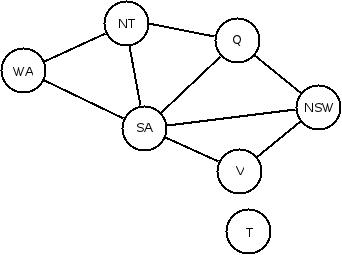
\includegraphics[scale=.5]{img/Australia.jpeg}
\caption{Esempio di grafo, colorazione della mappa australiana.}
\end{figure}

Si può dare una \emph{formulazione incrementale} di un CSP come se fosse un
problema di ricerca:
\begin{itemize}
\item[-]\textbf{Stato iniziale}: l'assegnamento vuoto $\{\}$ nel quale
nessuna variabile ha un valore assegnato.
\item[-]\textbf{Funzione successore}: assegna un valore ad una variabile
in modo  che
non violi alcun vincolo ad essa associato.
\item[-]\textbf{Test obiettivo}: verifica che l'assegnamento sia completo.
\item[-]\textbf{Costo di cammino}: costante per ogni passo.
\end{itemize}

Poiché una soluzione deve essere un assegnamento completo avrà almeno profondità
$n$, dove $n$ è il numero di variabili coinvolte. Per questo, per risolvere i
CSP sono molto utilizzati gli algoritmi di ricerca in profondità.

\`E quindi possibile definire una \emph{formulazione a stato completo} del
problema, nella quale ogni stato è un assegnamento completo che può soddisfare
i vincoli oppure no. Questo approccio è utilizzato negli algoritmi di ricerca
locale, nei quali viene assegnato un valore ad ogni variabile per lo stato
iniziale e normalmente la funzione successore cambia il valore di una variabile
alla volta.

\section{Un semplice esempio: colorazione di una mappa}
Si è definito formalmente un problema di soddisfacimento di vincoli e si è
quindi spiegato brevemente cosa significa risolverlo. A questo punto vediamo un
classico esempio: la colorazione di mappe geografiche.

La colorazione delle regioni di uno stato su una mappa geografica può essere
facilmente espresso mediante un CSP, prendiamo come esempio la mappa
dell'Australia (esempio trattato in \cite{intArt}).

\subsection{Definizione del problema}
Innanzitutto occorre stabilire qual'è il problema. Colorare le regioni di un
paese in modo che non si confondano significa che quelle adiacenti devono
avere colori differenti. Supponiamo di avere a disposizione solo tre colori:
rosso, verde e blu. Le regioni dell'Australia sono sette: Western Australia,
Northern Territory, South Australia, Queensland, New South Wales, Victoria
e l'isola della Tasmania. In figura \ref{figAustralia} si notano le varie
regioni sotto forma di nodi del grafo dei vincoli, gli archi rappresentano la
relazione di
confine tra regioni.

A questo punto abbiamo tutti gli elementi per ottenere un problema
$\mathbf{P} = \left\langle \mathbf{V}, \mathbf{D}, \mathbf{C}\right\rangle$
tale che:
\[
\mathbf{V} = \left\{ W_A, N_T, S_A, Q, N_{SW}, V, T \right\},
\]
\[
\mathbf{D} =  \left\{\textrm{rosso},\textrm{verde},\textrm{blu}\right\},
\]
in cui i vincoli appartenenti a $\mathbf{C}$, descritti dagli archi del grafo,
sono del tipo:
\[
\mathcal{C}_1 \leftarrow  W_A \neq N_T, \quad \mathcal{C}_2 \leftarrow  W_A
\neq S_A,\quad \ldots
\]

\subsection{Dalla definizione formale alla realizzazione in Java mediante
JSR-331}
Come già accennato nella sezione precedente la definizione formale di un
CSP e la sua soluzione sono concetti abbastanza generici da poter essere
applicati a qualunque sistema di risolutori o linguaggio di programmazione.

Tuttavia la sintassi può essere molto differente tra un linguaggio e l'altro, ma
anche tra un risolutore e un altro scritti nel medesimo linguaggio, la
specifica JSR-331 si prefigge di standardizzare tale sintassi mediante
la definizione di un'interfaccia. Vediamo come può essere rappresentato
il problema dell'Australia.

\begin{lstlisting}[language=Java,
                   caption = {\files{Australia.java}.}]
public class Australia {
  static final String[] colors = { "red", "green", "blue"};
...
}
\end{lstlisting}
Viene creata la classe \files{Australia} in cui verrà definito il problema
e la chiamata al risolutore di vincoli. L'array di stringhe rappresenta
il dominio delle variabili che verranno create.

\begin{lstlisting}[language=Java,
                   caption = {definizione delle variabili.},
                   frame = shadowbox]
static public void main(String[] argv) {
  try {
    Problem p = new Problem("Australia");
    // Variabili.
    int n = colors.length-1;
    Var WA   = p.variable("Western Australia",0, n);
    Var NT   = p.variable("Northern Territory", 0, n);
    Var SA   = p.variable("South Australia",0, n);
    Var Q    = p.variable("Queensland",0, n);
    Var NSW  = p.variable("New South Wales",0, n);
    Var V    = p.variable("Victoria",0, n);
    Var T    = p.variable("Tasmania",0, n);
\end{lstlisting}
In questa parte di codice viene creato il problema \files{p} chiamato
``Australia''
e vengono quindi create le variabili legate al problema (costruite dal
metodo \files{variable(nome, min, max)} della classe \files{Problem}).

Si noti che il dominio delle variabili è specificato nella chiamata del metodo
\files{variable}, ovvero ogni variabile ha dominio $[0, n-1]$, in cui $n$ è
la lunghezza del vettore dei domini. Le variabili si riferiscono in pratica agli
indici di tale vettore.

\begin{lstlisting}[language=Java,
                   caption = {definizione dei vincoli.},
                   frame = shadowbox]
    // Vincoli.
    p.post(WA, "!=", NT);
    p.post(WA, "!=", SA);
    p.post(NT, "!=", SA);
    p.post(NT, "!=", Q);
    p.post(SA, "!=", Q);
    p.post(SA, "!=", NSW);
    p.post(SA, "!=", V);
    p.post(Q, "!=", NSW);
    p.post(V, "!=", NSW);
\end{lstlisting}
La definizione dei vincoli avviene mediante il metodo
\files{post(Var, String, Var)}, sempre invocato sul problema. In questo caso
vengono specificati tutti i vincoli di disuguaglianza come specificato in figura
\ref{figAustralia}.

\begin{lstlisting}[language=Java,
                   caption = {ricerca della soluzione.},
                   frame = shadowbox]
Solution solution = p.getSolver().findSolution();
if (solution != null) {
  for (int i = 0; i < p.getVars().length; i++) {
    Var var = p.getVars()[i];
    p.log(var.getName() + " - " +
    colors[solution.getValue(var.getName())]);
  }
}
else
  p.log("no solution found");
\end{lstlisting}
Dopo aver trovato la soluzione, viene stampata mediante
un semplice algoritmo (che ovviamente non fa parte dello standard) e questo è
il risultato ottenuto con JSetL:
\begin{lstlisting}[caption = {la soluzione.},
                   frame = shadowbox]
Western Australia - red
Northern Territory - green
South Australia - blue
Queensland - red
New South Wales - green
Victoria - red
Tasmania - red
\end{lstlisting}
